\documentclass[12pt,english,brazil,a4paper,utf8,oneside]{utfpr-tcc}

% Este comando não é necessário: utilizei apenas para deixar o latex2rtf
% feliz (e descobrir a codificação do texto).
\usepackage[utf8]{inputenc}

% Suporte a figuras e subfiguras
\usepackage{graphics}
\usepackage{subfigure}

% Suporte a tabelas (principalmente do cronograma)
\usepackage{tabularx}
\usepackage{multirow}
\usepackage{array}
\usepackage{tabularx}
\usepackage{colortbl}
\usepackage{hhline}
\usepackage{xcolor}

% Elementos geralmente utilizados na tabela do cronograma
\newcommand{\fullcell}{\multicolumn{1}{>{\columncolor[gray]{0.5}}c}{}}
\newcommand{\fullcellline}{\multicolumn{1}{>{\columncolor[gray]{0.5}}c|}{}}
\newcommand{\mc}[3]{\multicolumn{#1}{#2}{#3}}
\newcommand{\y}{\rule{8pt}{4pt}}
\newcommand{\n}{\hspace*{8pt}} 

% Define o caminho das figuras
\graphicspath{{images/}}

% Dados do curso que não precisam de alteração
\university{Universidade Tecnológica Federal do Paraná}
\universityen{Federal University of Technology -- Paraná}
\universityunit{Departamento Acadêmico de Computação}
\address{Campo Mourão}
\addressen{Campo Mourão, PR, Brazil}
\documenttype{Monografia}
\documenttypeen{Monograph}
\degreetype{Graduação}


%%%%%%%%%%%%%%%%%%%%%%%%%%%%%%%%%%%%%%%%%%%%%%%%%%%%%%%%%%%%%%%%%%%%%%%%%%%%%
% Alterar daqui para baixo
%%%%%%%%%%%%%%%%%%%%%%%%%%%%%%%%%%%%%%%%%%%%%%%%%%%%%%%%%%%%%%%%%%%%%%%%%%%%%

% Dados do curso. Caso seja BCC:
\program{Curso de Bacharelado em Ciência da Computação}
\programen{Undergradute Program in Computer Science}
\degree{Bacharel}
\degreearea{Ciência da Computação}
% Caso seja TSI:
% \program{Curso Superior de Tecnologia em Sistemas para Internet}
% \programen{Undergradute Program in Tecnology for Internet Systems}
% \degree{Tecnólogo}
% \degreearea{Tecnologia em Sistemas para Internet}


% Dados da disciplina. Escolha uma das opções e a descomente:
% TCC1:
\goal{Proposta de Trabalho de Conclusão de Curso de Graduação}
\course{Trabalho de Conclusão de Curso 1}
% TCC2:
% \goal{Trabalho de Conclusão de Curso de graduação}
% \course{Trabalho de Conclusão de Curso 2}


% Dados do TCC (precisa alterar)
\author{Tiago Kenji Umemura}  % Seu nome
\title{Uma ferramenta para monitoramento da entropia de mudança e sua relação com métricas de software} % Título do trabalho
\titleen{} % Título traduzido para inglês
\advisor{Prof. Dr. Igor Scaliante Wiese} % Nome do orientador. Lembre-se de prefixar com "Prof. Dr.", "Profª. Drª.", "Prof. Me." ou "Profª. Me."}
% \coadvisor{} % Nome do coorientador, caso exista. Caso não exista, comente a linha.
\depositshortdate{2016} % Ano em que depositou este documento

% Dados da ficha catalografica. Ela é opcional, mas é uma boa ideia inserí-la. Exemplos para geração (http://fichacatalografica.sibi.ufrj.br/)
\fichacatautor{}  % Nome conforme citado (ou seja, no formato "Sobrenome, Nome").
\fichacatbib{Biblioteca da UTFPR de Campo Mourão} % Não alterar
\fichacatpum{M488} % Código Cutter-Sanborn. Use a primeira letra do sobrenome seguido do número conforme as primeiras letras do sobrenome e a tabela http://www.amormino.com.br/cutter-sanborn/cutter1.html
\fichacatpalcha{} % Assuntos do trabalho. Cada item deve ser enumerado e separado por ponto: 1. xxx. 2. yyy. 3. zzz.
\fichacatpdois{} % Deixar em branco


\begin{document}
	
\frontmatter
\maketitle

\begin{resumo}

% TODO: se possível, escreva um resumo estruturado. Para TCC 1, o resumo estruturado teria os seguintes elementos:
\textbf{Contexto:} A entropia de mudança é uma medida para indicar o quanto um software sofre alterações em um determinado período de tempo. Estudos mostraram que o aumento da entropia pode causar desordem no processo de desenvolvimento podendo levar ao aumento no número de defeitos do software. Porém não foi analisado a relação da entropia com uma grande quantidade de métricas de software e além disso não há uma ferramenta que monitore a relação entre a entropia de mudança e métricas de softwares, como por exemplo, número de autores que modificaram um arquivo, número de \textit{commits}, \textit{authorship} e \textit{ownership}\\
\textbf{Objetivo:} Implementar uma ferramenta que possibilite o monitoramento da entropia e das métricas de softwares de projetos armazenados no Github para ajudar os desenvolvedores no gerenciamento de projeto. \\
\textbf{Método:} A ferramenta é dividida em coleta de dados, cálculo da entropia, cálculo das métricas, análise estatística, visualização de dados e avaliação.
Na coleta de dados os dados serão extraídos do GHTorrent e da API Github e após a coleta será realizado o cálculo da entropia e das métricas de software utilizando principalmente a ferramenta Change Metrics. Na etapa de análise estísticas será feito a comparação e a correlação entre as métricas e em seguida será gerado um relatório sobre os resultados para o usuário. Na etapa de visualização de dados, a entropia de mudança será exibida utilizando o \textit{Treemapping} e serão contruídos gráficos que mostram o comportamento das métricas ao longo do tempo. Para a avaliação da ferramenta será convidado desenvolvedores para testar a ferramenta e depois serão feitos questionários sobre a usabilidade da ferramenta para esses desenvolvedores.\\
\textbf{Resultados esperados:} É esperado que a ferramenta ajude os desenvolvedores a gerenciar melhor os projetos oferecendo relatórios estatísticos e visualizações da relação da entropia com as métricas sociais, de processo e de autoria.
% ou, para TCC 2:
% \textbf{Contexto:} \\
% \textbf{Objetivo:} \\
% \textbf{Método:} \\
% \textbf{Resultados:} \\
% \textbf{Conclusões:}

% Palavras-chaves, separadas por ponto (tente não definir mais do que cinco)
\palavraschaves{Entropia. Fatores Sociais. Defeitos.}
\end{resumo}

%quais fatores tem incluencia na entropia (main quest)
%visualização de indicadores dos fatores com a entropia (side quest)

% Caso seja TCC 2, precisa traduzir o resumo e as palavras-chaves para inglês:
% \begin{abstract}
% \textbf{Context:}
% \textbf{Objective:}
% \textbf{Method:}
% \textbf{Results:}
% \textbf{Conclusions:}

% Palavras-chaves em inglês, separadas por ponto.
% \keywords{}
% \end{abstract}



% Listas (opcionais, mas recomenda-se a partir de 5 elementos)
\listoffigures
\listoftables

% Sumário
\tableofcontents

\mainmatter
% TODO: incluir arquivos latex com os capítulos
 \chapter{Introdução}

Os artefatos de softwares são modificados ao longo do tempo e nesse processo a qualidade do software tende a piorar, uma vez que existe a necessidade da mudança contínua de requisitos durante a evolução do software \cite{Hassan:2009:PFU:1555001.1555024}.

Para quantificar o impacto das mudanças contínuas os pesquisadores tem utilizado o conceito de entropia de mudança \cite{Hassan:2009:PFU:1555001.1555024}. Esta medida pode ser obtida a partir do número de mudanças que ocorrem em um projeto ou arquivo em um determinado período de tempo. \citeonline{Hassan:2009:PFU:1555001.1555024} observou que maior quantidade de mudanças está relacionada com o aumento do valor da entropia e consequentemente está relacionado com maior tendência do software apresentar defeitos. \citeonline{Canfora2014} analisou a relação entre a entropia e atividades de desenvolvimento, como a refatoração, padrões de projetos e a quantidade de desenvolvedores que mudam um determinado arquivo.

Dada a importância da entropia de mudança, é necessário que desenvolvedores e gerentes possam monitorar os valores de entropia dos arquivos e a possível relação do aumento da entropia com as métricas de software. Não foram encontrados estudos que tenham propostos ferramentas que possibilitem o monitoramento da relação da entropia com as métricas de softwares.

Portanto não existe uma ferramenta que possibilite os desenvolvedores e os gerentes monitorarem os efeitos da entropia e sua relação com métricas sociais, de autoria e de processo.

Diante desse contexto, sabe-se que o desenvolvimento de software é uma tarefa sóciotécnica, pois é essencial a comunicação entre os desenvolvedores para coordenar as atividades de desenvolvimento durante a evolução do software e uma ferramenta poderia monitorar os aspectos sociais e técnicos do projeto para auxiliar os desenvolvedores. Assim o objetivo deste trabalho é construir uma ferramenta que monitora os valores de entropia e a sua relação com as métricas sociais (número de comentários em \textit{Pull Request} e número de \textit{Pull Request}), de autoria de mudança (\textit{authorship}, \textit{ownership} e experiência) e métricas de processo (quantidade de \textit{commits}, quantidade de defeitos, quantidade de linhas removidas, quantidade de linhas adicionadas, \textit{Code Churn}, quantidade de refatorações, \textit{max change set} e \textit{average change set}).

A ferramenta irá gerar relatórios estatísticos sobre a entropia e as métricas e fornecerá a visualização desses dados para auxiliar os desenvolvedores na tomada de decisões durante o desenvolvimento de um projeto. Na visualização de dados será utilizado o \textit{Treemapping} para  mostrar quais arquivos do projeto possuem maior entropia e para as métricas de software serão utilizados gráficos que mostrem os valores das métricas ao longo do tempo.

Para avaliar a ferramenta serão convidados desenvolvedores que responderão um questionário sobre as funcionalidades e usabilidade da ferramenta.  

Esta proposta está organizada da seguinte forma. O capítulo 2 apresenta as definições das métricas sociais, de processos e os trabalhos relacionados. O capítulo 3 apresenta a proposta de construção da ferramenta, como a ferramenta será validada e uso da ferramenta. O capítulo 4 apresenta o cronograma.
 \chapter{Referencial Teórico}
Este capítulo apresenta os conceitos de entropia, métricas socias e métricas de processo e indicadores de qualidade.

\section{Entropia de mudança}
A entropia de \citeonline{Shannon:2001:MTC:584091.584093} é uma medida para mensurar a incerteza associada a uma variável que quantifica uma informação contida em uma mensagem produzida por um emissor de dados. É utilizada para determinar a quantidade de bits necessários para identificar unicamente um distribuidor de dados, assim quanto maior a entropia maior a incerteza para identifica-lo. A partir disso foi criado a entropia de mudança com o objetivo de calcular o quanto um código está mudando durante um determinado período de tempo. 

A entropia de mudança introduzida por \citeonline{Hassan:2009:PFU:1555001.1555024} considera que o software é o emissor de dados e as modificações realizadas são os dados a serem considerados. É uma medida para mensurar a quantidade de mudanças que ocorreram em um determinado espaço de tempo em um arquivo de um projeto, as mudança consideradas podem ser obtidas a partir da quantidade de linhas modificadas em um intervalo de tempo ou utilizando número de commits. Hassan também mostrou que alta entropia está relacionada a maior tendência do projeto apresentar falhas.

A entropia de mudança é definida como:

\begin{equation}
H(S) = {\sum\limits_{n=1} }\frac{chg(f_i)}{chg(S)}log_2(\frac{chg(f_i)}{chg(S)})
\end{equation}

\subsection{Trabalhos Relacionados}
A pesquisa de \citeonline{Canfora2014} relaciona a entropia de mudança com características do software e atividades de desenvolvimento. As características analisadas foram: refatoração, número de commiters, padrões de projetos e nome de tópicos no projeto. Na pesquisa foram analisados projetos nos sistemas ArgoUML, Eclipse-JDT, Mozilla e Samba em um período de cerca de 10 anos e foi mostrado como esses fatores se relacionam com a entropia, que por consequecia impacta a qualidade do software. Os resultados de Canfora indicam que a entropia de mudança varia conforme o número de desenvolvedores aumentam, sendo que diferentes sistemas de controle de versão apresentam variações diferentes na entropia.

Nesse estudo, o método para extração de dados é dividido em 6 passos: extração das métricas de mudança do sistema de controle de versão, cálculo da entropia de mudança, identificação das mudanças relacionadas a refatoração, contar número de autores que contribuem para o projeto, identificação dos padrões de projetos e por último é necessário identificar os tópicos que são descritos na mensage de cada commit. 

Após a extração dos dados é feito a análise desses dados. No caso da refatoração, é feito a comparação do valor da entropia antes e depois da refatoração.

\section{Métricas}
\subsection{Métricas de autoria}
Esta seção apresenta métricas para calculadas a partir das atividades dos usuário em cada projeto.

\subsubsection{Authorship}
Authorship é uma medida para mensurar o quanto um desenvolvedor contribuiu para um determinado módulo de software e o ownership é o autor com maior authorship, assim um módulo de software pode apresentar ownership forte ou distribuído entre os contribuidores.

Essas duas medidas podem ser obtidas de várias formas: contando número de arquivos que o desenvolvedor modificou, número de commits e outra possibilidade é contar número de linhas modificadas pelo contribuidor, também chamada de code churn\cite{Munson:1998:CCM:850947.853326}.

No trabalho de Greiler e Kim Herzig\cite{Greiler} é feito um estudo para relacionar Ownership com a qualidade do código. Para medir a qualidade do código é considerado o número de bugs que foram corrigidos, número de diretórios e arquivos defeituosos e o Ownership é medido considerando número de contribuidores de um arquivo e também é verificado se existe um contribuidor principal, nesse caso a medida foi calculada com base no número de commits do autor em relação ao total de commits para aquele componente. Também foi mostrado que módulos com ownership fraco tendem a apresentar mais defeitos. Nesse mesmo trabalho foi estudado quatro diferentes software para Windows e é possível observar que nos sistemas analisados a métrica de ownership está correlacionado com número de defeitos. Isso é observado na análise feita tanto em nível de arquivo quanto em nível de diretório.  
Essa pesquisa mostrou que o número de contribuidores e a porcentagem de mudanças aplicadas pelo ownership são bons indicadores de qualidade , mostrando que há relação entre ownership e a qualidade de um projeto apesar da quantidade de erros também depender do tamanho do projeto.

Na pesquisa realizada por \citeonline{Rahman2011} é analisado a relação entre o número de autores com o ownership e com a qualidade do código. O authorship é calculado utilizando o número de linhas modificadas no código pelo desenvolvedor dividido pelo número total de linhas do arquivo, e o autor com a maior contribuição é denomidado ownership. Também é definido implicated code, que é o código modificado quando é corrigido um determinado erro no módulo de software. O trabalho de Rahman investiga a relação entre ownership, authorship e experience com implicated code. Para cada linha de código modificado é utilizado o comando blame para identificar o autor responsável por essa mudança. O resultado fornece evidências indicando que implicated code tende a ser mais frequentemente gerado por poucos autores, vários fragmentos de códigos modificados tem apenas um único autor.

O artigo de \citeonline{Foucault2015} também estuda como o ownership impacta na qualidade do código. Nele os contribuidores são classificados como owner, minor e major. Owner é o contribuidor com maior valor de contribuição, minor o desenvolvedor que contribuiu com menos de 5\% e major contribuiu com mais de 5\%. Após medir as métricas é comparado o número de erros com o a medida de ownership.

Além disso também há pesquisas\cite{Thongtanunam} que analisaram a diferença entre a contribuição de code authoring e reviewing e como a atividade de code reviewing afetam projetos com vários autores que contribuem pouco o que ajuda a compreender melhor o impacto do ownership na qualidade do código.

\subsubsection{Ownership}

\subsubsection{Experience}
A experience do desenvolvedor influência na produtividade do mesmo e na qualidade do código produzido como foi mostrado em outras pesquisas\cite{Rahman2011}\cite{10.2307/2634607} e quanto mais o desenvolvedor trabalha em diferentes componentes do sistema maior será a sua experience.

Já foi feito pesquisas\cite{Rahman2011} mostrando a relação entre experience e qualidade do código além disso a experience é dividida em dois tipos: a experience especializada e experience geral. A experience especializada é medida considerando o quanto um indivíduo contribui em um determinado arquivo e a experiência geral é medida conseiderando um projeto inteiro.

A experience é a medida para calcular o nível de experiência do contribuidor, essa medida é computada analisando o número de linhas\cite{Rahman2011} deltas comitadas pelo contribuidor em determinado espaço de tempo. Além disso Rahman já mostrou que experiência especializada leva a produzir códigos com menor número de erros e ainda não foi possível concluir que a experiência geral contribui para aumentar a qualidade. No trabalho de Rahman foi correlacionado implicated code com experience.

\subsection{Métricas Sociais}
\subsubsection{Quantidade de mensagens trocadas}

\subsection{Métricas de processo}
Esta seção apresenta as métricas extraídas utilizando a ferramenta Change Metrics desenvolvida por Maurício Aniche.
\subsubsection{Quantidade de autores}
Esta métrica é utilizada para contar a quantidade de autores diferentes que contribuem com o projeto.
\subsubsection{Quantidade de commits}
A quantidade de commits representa o nível de atividade do projeto em termos de número de commits feitos. È calculado o número de commits do projeto em um certo perído de tempo. 
\subsubsection{Quantidade de defeitos}
A quantidade de defeitos será calculado com o número de issues do projeto que foram criadas em uma determinada data. Essa data é obtida a partir do GHTorrent no campo created\_at.
\subsubsection{Idade do repositório}
A métrica idade do repositório representa o tempo de existência do projeto. O cálculo é utilizado medindo a diferença de tempo entre o primeiro e último commit.

canfora e hassan
 \chapter{Proposta}
Nos estudos realizados por \citeonline{Hassan:2009:PFU:1555001.1555024} e \citeonline{Canfora2014} foram analisados a relação da entropia de mudança com a qualidade do projeto e algumas métricas de software, como por exemplo, número de contribuidores, no entanto, não há uma ferramenta que monitore a entropia e a relação com métricas sociais, de autoria e de processo.

Portanto o objetivo deste trabalho é implementar uma ferramenta que monitore o valor da entropia de mudança e sua relação com as métricas sociais, de autoria e de processo dos projetos. A ferramenta terá seis módulos que serão apresentados na figura 3.1 e as funcionalidades são apresentadas na figura 3.2:

\begin{figure}[H]
	\captionsetup{justification=centering}
	\includegraphics[width=\linewidth]{fluxogramaTCC.png}
	\caption{Fluxograma do funcionamento da ferramenta}
	\label{figura:fluxogramaimagem}
\end{figure}

\begin{figure}[H]
	\captionsetup{justification=centering}
	\includegraphics[width=\linewidth]{DiagramaDeCasoDeUso.png}
	\caption{Diagrama de caso de uso da ferramenta}
	\label{figura:diagramacaso}
\end{figure}

\section{Coletar dados}
O módulo de coleta de dados é responsável pela extração de dados dos projetos do Github e Git que serão persistidos em um banco de dados local. Os dados serão obtidos utilizando o GHTorrent\footnote{GHTorrent é uma ferramenta que monitora os eventos públicos do Github, para cada evento é armazenado o seu conteúdo e as resposta JSON são armazenadas em um banco de dados MongoDB e também no MySQL} e a API Github\footnote{API Github permite coletar dados sobre os repositórios do Github, onde os dados são recebidos no formato JSON. A documentação da API pode ser encontrada no endereço: https://developer.github.com/v3/}.

Utilizando a base de dados MySQL do GHTorrent será extraído dados sobre os \textit{commits}, \textit{issues}, \textit{Pull Requests} e contribuidores do projeto. Além disso, será feito o clone das versões dos projetos selecionados utilizando o comando \textit{git log}, \textit{git clone} e \textit{git reset}. 

\section{Calcular entropia}
Este módulo realiza o cálculo da entropia de cada arquivo do projeto no período que o usuário informar. O valor da entropia será determinado utilizando como medida o número de commits que o arquivo teve durante um período de tempo selecionado pelo usuário. Para o cálculo da entropia é necessário medir a diferença entre o número total de commits de duas versões diferentes do projeto, e assim, obter o número de commits que cada arquivo teve entre uma versão e outra.

\section{Calcular métricas}
O módulo de cálculo das métricas irá realizar o cálculo após a extração dos dados no módulo de coleta de dados. Nessa etapa o usuário deverá informar quais métricas ele deseja calcular e uma data anterior a data atual. O período definido será entre a data atual e a data definida pelo usuário e as métricas serão calculadas de 15 em 15 dias.

Para o cálculo das métricas de processo será utilizada a ferramenta Change Metrics. Para executá-la é necessário três parâmetros: o projeto git, o arquivo csv onde serão armazenados os dados e tipo do projeto que pode ser \textit{all} ou \textit{single}. O comando para executar a Change Metrics é: java -jar <tool.jar> projeto arquivo.csv single. 

A forma como as métricas serão calculadas estão descritas na tabela 3.1. 

\begin{table}[H]
\centering
\caption{Tabela de cálculo das métricas}
\label{cálculometricas}
\begin{tabular}{|p{4cm}|p{12cm}|}
\hline
Métrica                             & Descrição do cálculo                                                                        \\ \hline
Authorship                          & Média da quantidade de commits considerando todos os contribuidores                         \\ \hline
Ownership                           & Maior valor da métrica de authorship                                                        \\ \hline
Experiência                         & Média da quantidade de linhas modificadas no arquivo por todos os contribuidores            \\ \hline
Pull Request fechados por arquivo   & Contagem do número de Pull Request fechados relacionados a um determinado arquivo           \\ \hline
Pull Request abertos por arquivo    & Contagem do número de Pull Request abertos relacionados a um determinado arquivo            \\ \hline
Comentários em Pull Request aberto  & Contagem do número de comentários em todos os Pull Request abertos relacionados ao arquivo  \\ \hline
Comentários em Pull Request fechado & Contagem do número de comentários em todos os Pull Request fechados relacionados ao arquivo \\ \hline
Média do tempo de vida de \textit{Pull Request} & Será calculado a diferença no tempo entre a abertura e o fechamento do \textit{Pull Request} \\ \hline
Quantidade de commits               & Calculado utilizando a ferramenta Change Metrics                                        \\ \hline
Quantidade de defeitos              & Calculado utilizando a ferramenta Change Metrics                                            \\ \hline
Idade do arquivo                    & Calculado utilizando a ferramenta Change Metrics                                            \\ \hline
Quantidade de linhas removidas      & Calculado utilizando a ferramenta Change Metrics                                            \\ \hline
Quantidade de linhas adicionadas    & Calculado utilizando a ferramenta Change Metrics                                            \\ \hline
Code Churn                          & Calculado utilizando a ferramenta Change Metrics                                            \\ \hline
Quantidade de refatorações          & Calculado utilizando a ferramenta Change Metrics                                            \\ \hline
Max Change set                      & Calculado utilizando a ferramenta Change Metrics                                            \\ \hline
Average Change set                  & Calculado utilizando a ferramenta Change Metrics                                            \\ \hline
\end{tabular}
\end{table}

\section{Gerar relatório de análise estatística}
Como foi feito na pesquisa de \citeonline{Canfora2014}, para analisar a relação da entropia e as métricas de software serão utilizados os métodos estatísticos de \textit{Wilcoxon}, \textit{ANOVA} e \textit{Cliff's Delta}, onde todos os testes serão feitos no ambiente estatístico R com nível de significância de 95\%.

O teste de \textit{Wilcoxon} é um método não paramétrico para comparação de duas amostras com o objetivo de verificar se existem diferenças significativas entre elas. E para mensurar a diferença entre as amostras é utilizado o \textit{Cliff's Delta}, uma medida de tamanho de efeito não paramétrico, que por exemplo, pode ser utilizada para mensurar a diferença no valor da entropia de mudança entre dois intervalos de tempo.

A \textit{ANOVA} (Análise de Variância) é usada para verificar se a média de duas ou mais populações são iguais e determina se as diferenças entre as médias amostrais sugerem diferenças significativas entre as médias das populações ou se essas diferenças decorrem apenas da variabilidade implícita de cada amostra. O método \textit{ANOVA} irá ser utilizado para analisar a interação entre a entropia de mudança e as métricas de software descritas na seção anterior. 

Após a análise estatística, será gerado um relatório para informar o usuário quais métricas apresentam maior relação com a entropia e quais arquivos possuem maior entropia, por exemplo, selecionando os arquivos com valor de entropia maior que a mediana da entropia de todos os arquivos.

\section{Gerar Visualização}
Este módulo permite o usuário utilizar filtros para escolher quais métricas ele deseja visualizar. Para visualização será utilizado o \textit{Treemapping}, \textit{Heat Map} e séries temporais.

O \textit{treemapping} é uma forma de visualização de dados de forma hierárquica utilizando retângulos aninhados. Na ferramenta o \textit{Treemapping} será utilizado para visualizar o valor da entropia dos arquivos do projeto, onde cada retângulo representará um arquivo e o tamanho desse retângulo representa o valor da entropia, quanto maior a entropia maior será o retângulo. O usuário poderá escolher qual período de tempo ele deseja visualizar o valor da entropia e também poderá comparar esse valor entre dois peŕiodos diferentes, sendo que o valor da entropia é calculado de 15 em 15 dias.

\begin{figure}[H]
	\captionsetup{justification=centering}
	\centerline{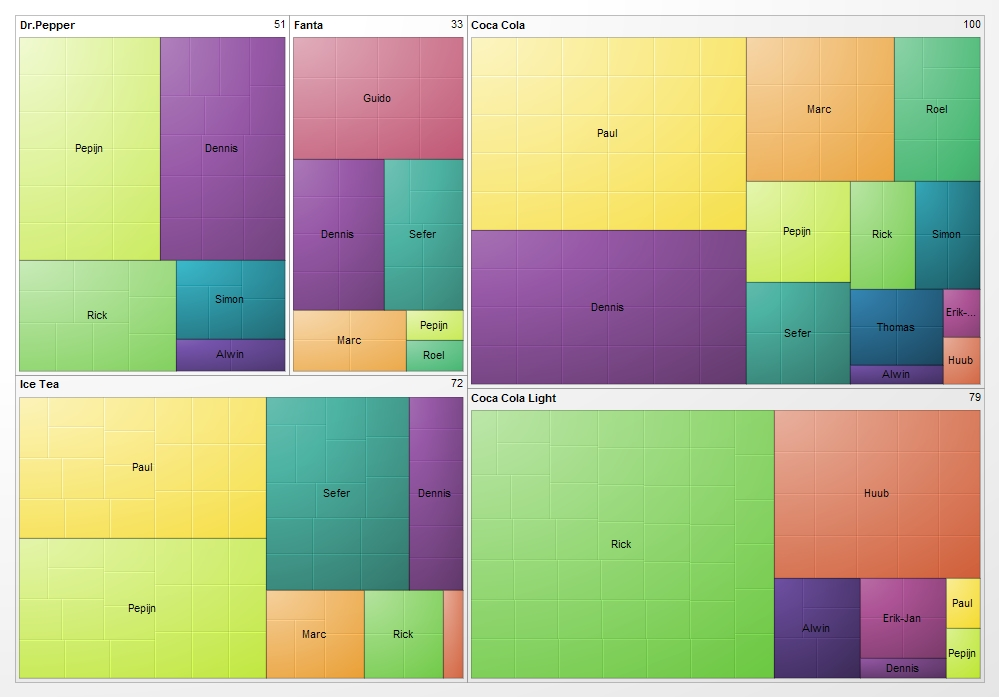
\includegraphics[scale=0.2]{treemap.jpg}}
	\caption{Exemplo de visualização utilizando Treemapping.}
	\label{figura:visaometodo}
\end{figure}

O \textit{Heat Map} é uma representação gráfica que utiliza cores para mostrar as relações entre os valores dos dados. Essa visualização será utilizada em forma de matriz, onde as linhas e colunas representarão as métricas e as cores nas intersecções representarão o nível de correlação entre as métricas e entre as métricas e a entropia de mudança. A cada período de 15 dias será gerado um \textit{Heat Map}.

\begin{figure}[H]
	\captionsetup{justification=centering}
	\centerline{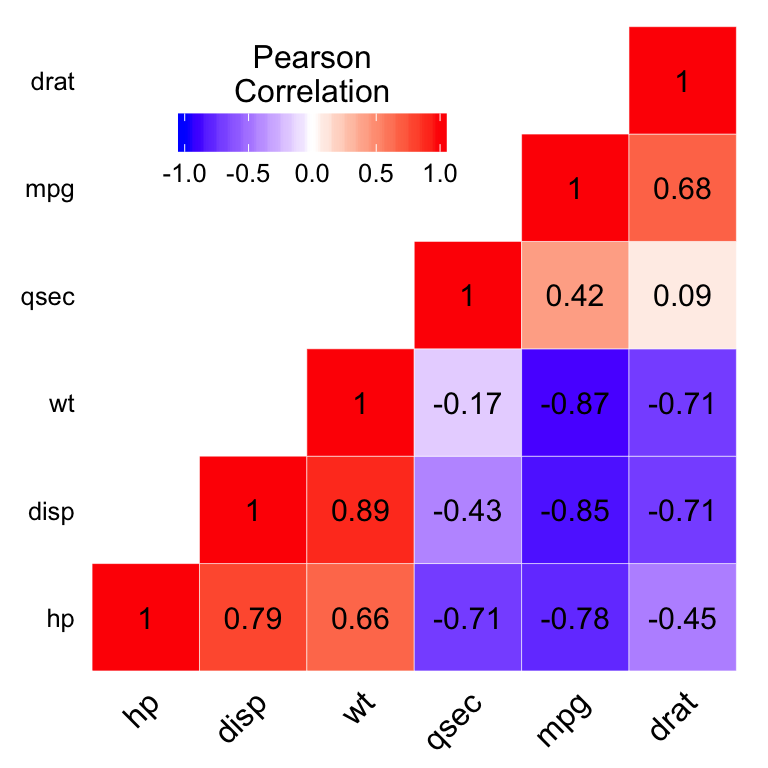
\includegraphics[scale=0.3]{heatmap.png}}
	\caption{Exemplo de Heat Map com matriz}
	\label{figura:heatmap}
\end{figure}

Será utilizado um gráfico de séries temporais para mostrar a evolução das métricas ao longo do tempo como mostra as figura 3.4. O eixo x do gráfico representa o tempo e o eixo y representa o valor da métricas, sendo que o tempo está dividido a cada 15 dias.

\begin{figure}[H]
	\captionsetup{justification=centering}
	\centerline{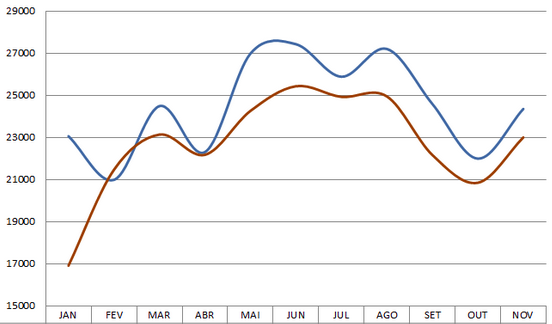
\includegraphics[scale=0.5]{metricaex.png}}
	\caption{Exemplo de gráfico de duas métricas ao longo do tempo}
	\label{figura:exmetrica}
\end{figure}

\section{Avaliar a ferramenta}
Para a avaliação, a ferramenta será configurada para 10 projetos e serão convidados desenvolvedores para utilizá-la, onde os desenvolvedores deverão realizar tarefas sobre as funcionalidades da ferramenta. As tarefas são descritas nos cenários apresentados a seguir:

Cenário 1: O desenvolvedor poderá escolher o período de tempo em que ele deseja analisar o projeto e quais filtros (métricas) ele deseja calcular. Após definir o período e os filtros, será gerado um gráfico de duas dimensões mostrando o comportamento das métricas ao longo do tempo. 

Cenário 2: O desenvolvedor poderá consultar o valor da entropia de cada arquivo após selecionar um período de 15 dias. O valor da entropia será mostrado por meio do \textit{Treemap} do projeto, onde cada retângulo representará um arquivo e o tamanho do retângulo representará o valor da entropia nesse arquivo. Ao clicar no \textit{Treemap} será gerado um relatório que irá conter informações sobre quais arquivo possuem maior entropia e portanto merecem maior atenção do desenvolvedor.

Cenário 3: O desenvolvedor poderá escolher um período (15 dias) e analisar a correlação entre as métricas e entre a entropia e as métricas utilizando o \textit{Heat Map}. Clicando no \textit{Heat Map} será gerado um relatório mostrando quais métricas possuem maior nível de correlação sugerindo que as maiores correlações influenciam no aumento da entropia.

Cenário 4: O desenvolvedor poderá comparar os valores da entropia e das métricas em dois períodos diferentes. Dois \textit{Treemaps} serão apresentados, um para cada período selecionado, para exibir os valores da entropia de cada arquivo do projeto e será apresentado uma tabela com os valores das métricas para cada período selecionado.

Cenário 5: O desenvolvedor ao gerar o \textit{Treemap} de um projeto durante um período poderá ter acesso a mais informações de cada arquivo do projeto. Ao clicar em um dos retângulos que representa um arquivo, o desenvolvedor terá acesso a um relatório com informações sobre quais métricas possuem maior correlação com a entropia daquele arquivo.

Após a realização das tarefas, os desenvolvedores responderão um questionário sobre a usabilidade da ferramenta. O questionário irá conter questões sobre a visualização de dados e o relatório estatístico para avaliar se a ferramenta auxilia o desenvolvedor na tomada de decisões do projeto. O questionário é composto por perguntas abertas e perguntas utilizando a escala Likert:

\begin{enumerate}
  \item Houve dificuldades para gerar o \textit{Treemap} do valor da entropia de um determinado período? (Escala Likert)
  
  \item Houve dificuldade para gerar o \textit{Heat Map}? (Escala Likert)
  
  \item Houve dificuldades para gerar os gráficos? (Escala Likert)
  
  \item O relatório estatístico sobre o valor da entropia nos arquivos é relevante para o desenvolvimento do projeto?
  
  \item A visualização dos valores da entropia de mudança utilizando \textit{Treemapping} é de fácil compreensão? (Escala Likert)
  
  \item A visualização de \textit{Heat Map} utilizada para analisar a correlação é de fácil compreensão? (Escala Likert)
  
  \item A correlação entre o valor da entropia e os valores das métricas é relevante para o desenvolvimento do projeto?
  
  \item Os gráficos de duas dimensões para analisar o histórico dos valores da métrica são importantes para tomar decisões no desenvolvimento do projeto?
\end{enumerate}
 \chapter{Cronograma}
\begin{table}[]
\centering
\caption{Tabela do cronograma}
\label{cronograma}
\begin{tabular}{|l|l|l|l|l|l|}
\hline
Módulos Ferramenta                     & Jan & Fev & Mar & Abr & Jun \\ \hline
Coletar dados                          & X   &     &     &     &     \\ \hline
Calcular entropia                      &     & X   &     &     &     \\ \hline
Calcular métricas                      &     & X   &     &     &     \\ \hline
Gerar Relatório de Análise Estatística &     &     & X   &     &     \\ \hline
Visualizar Dados                       &     &     &     & X   &     \\ \hline
Avaliar Ferramenta                     &     &     &     &     & X   \\ \hline
\end{tabular}
\end{table}

\bibliographystyle{abnt-alf}
\bibliography{main} % geração automática das referências a partir do arquivo main.bib

\backmatter
\end{document}
